% Analyse
\section{Analyse}

% User Szenarien
\subsection{User Szenarien}

Um die Anforderungen an die App genauer zu definieren, wurden im Vorfeld des Projektes einige Szenarien erstellt.
Gegen diese Szenarien kann die finale Applikation später getestet werden.

\subsubsection{Szenario 1: Zeitvertreib an der Bushaltestelle}

Simon muss 15 Minuten an der Bushaltestelle auf den nächsten Bus warten.
Um sich die Wartezeit zu verkürzen, nimmt er sein Smartphone hervor und startet die \textsc{Kort}-Applikation.

Die App hat ihn bereits lokalisiert und zeigt ihm offene OpenStreetMap-Aufträge, wahlweise als Liste oder auf der Karte, in der Nähe an.
Für die Aufträge werden Simon verschiedene Belohnungen angeboten, je nach Schwierigkeitsgrad der Aufgabe.

Simon entscheidet sich für einen Auftrag mit mittlerer Belohnung.
Die App zeigt ihm den Weg zum Auftrag und erklärt was zu tun ist. Beim Auftrag handelt es sich um einen fehlenden Strassennamen.

Als Simon vor Ort ist, findet er sehr schnell ein Strassenschild.
Er gibt den Namen in der App ein wofür er bereits 10 Punkte erhält.
Da er zusätzlich sogar noch Foto hochlädt, bekommt er noch 5 Bonuspunkte.

Der Auftrag ist somit für ihn erledigt was ihm entsprechend von der App mitgeteilt wird.
Danach verschwindet der Auftrag auch aus seiner Auftragsliste und von der Karte.

\textbf{Ziele}
\begin{itemize}
\item Zeitvertreib
\item Punkte sammeln
\item Daten verbessern
\end{itemize}

\subsubsection{Szenario 2: Validieren}

Andy sitzt im Zug und langweilt sich. Er öffnet die \textsc{Kort}-App im Indoor-Modus und sieht sich die Liste der zu validieren Bugfixes an. Er sortiert die Liste um diejenigen Einträge zu sehen, welche nur noch einen Review benötigen um zu OpenStreetMap gesendet zu werden.

Er öffnet einen Bugfix für einen fehlenden Strassennamen in der Umgebung. Er kennt zwar die Gegend ist sich aber nicht 100\% sicher ob der Name stimmt. Um sicherzugehen öffnet er das Bild, welches dem Bugfix angehängt ist. Das Bild zeigt ein Strassenschild, welches mit dem eingegeben Namen übereinstimmt. Andy bestätigt somit die Änderung und schliesst den Bug damit ab.

\textbf{Ziele}
\begin{itemize}
\item Schnell und einfach geeignete Einträge zum Validieren finden
\item Qualität der Änderungen sicherstellen
\end{itemize}

\subsubsection{Szenario 3: Erster Kontakt zur App}

Über den Kurznachrichtendienst Twitter sieht Monika, dass Ihre Kollegin gerade ein \textsc{Kort}-Konto erstellt hat.
Als sie auf den Link klickt öffnet sich ihr Browser und die App wird angezeigt.
Da es sich um ihren ersten Besuch auf der Seite handelt, wird ihr kurz erklärt um was es geht.

Danach sieht sie die Karte mit den vorhandenen Fehlereinträgen.
Bevor sie einen Eintrag bearbeiten kann, muss sie sich anmelden.
Sie wählt dazu einen Benutzernamen und wird anschliessend auf die Seite von Google weitergeleitet, um sich anzumelden.
Nach dem erfolgreichen Login wird Monika zurück zur \textsc{Kort}-App geleitet wo sie beginnen kann die ersten Aufträge zu erfüllen.

\textbf{Ziele}
\begin{itemize}
\item Direkt ersichtlich was die App kann
\item Schneller Einstieg
\item Einfache Anmeldung
\item Benutzerführung durch die Funktionen
\end{itemize}

\subsubsection{Szenario 4: Highscore-Anwärter}

Edi benutzt schon seit einiger Zeit die \textsc{Kort}-App und hat sich in seinem Revier bereits auf Platz 2 der Highscore-Liste geschafft.
Seine Rangierung überprüft er regelmässig auf der Highscore-Liste in der App.

Heute möchte er endlich die Spitze erklimmen und den "Leader"-Badge erhalten.
Dazu hat er sich einige Aufträge ausgesucht, welche er der Reihe nach abarbeiten will.
Bei jedem Auftrag sieht Edi wieviele Punkte er sammeln kann.

Nachdem er den 5. Auftrag erfolgreich erledigt hat, erhält er eine Benachrichtigung, dass der den "`Leader"'-Badge erhalten hat.
Auch in der Highscoreliste steht Edi nun zuoberst.

\textbf{Ziele}
\begin{itemize}
\item Einfach mehrere Aufträge nacheinander ausführen
\item Badges sammeln
\item Highscoreliste anzeigen und Erster werden
\end{itemize}

% Paper-Prototype
\subsection{Paper-Prototype}
% Subfigure counter zuruecksetzen
\setcounter{subfigure}{0}

Vor der Implementation der Oberfläche wurde ein Paper-Prototype des GUI-Designs erstellt.
Der Prototype besteht aus vier Hauptmasken und einem Overlay für den Login.

\subsubsection{Overlay: Login}
Beim ersten Starten der \gls{WebApp} erhält man die Möglichkeit sich über verschiedene Dienste anzumelden.
Beim Klick auf den jeweiligen Anbieter wird man zu diesem Weitergeleitet und kann sich dort anmelden.

\begin{figure}[H]
\subfigure[Login - Anbieterauswahl]{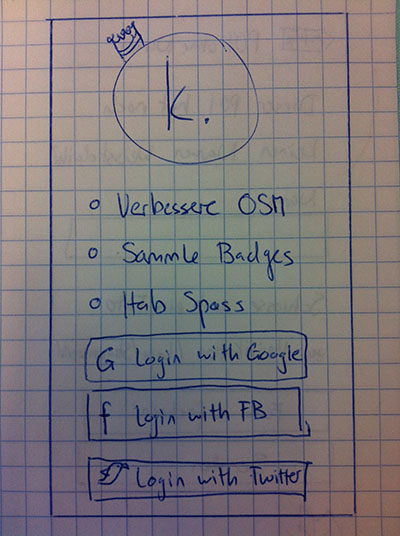
\includegraphics[width=0.43\textwidth]{images/paperprototype/kort-pp-startscreen}}
\hfill
\subfigure[Login - Loginformular des jeweiligen Anbieters]{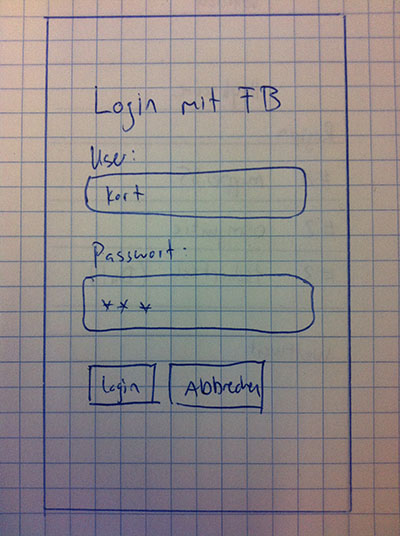
\includegraphics[width=0.43\textwidth]{images/paperprototype/kort-pp-login}}
\end{figure}

\subsubsection{Maske: Aufträge}
Ist der Login erfolgt erscheint die Maske mit den Aufträgen.
Darauf ist werden die bestehenden Fehler auf einer Karte angezeigt.
Es werden jeweils nur die Fehler angezeigt, welche sich in unmittelbarer Nähe vom eigenen Standort befinden.
Die Fehler werden mit einer Markierung auf der Karte dargestellt.

Durch Anklicken einer solchen Markierung öffnet sich die Detailansicht des Fehlers, worin sich der Fehler direkt beheben lässt.
Neben der Möglichkeit einen Lösungstext einzugeben, soll es auch möglich sein ein Beweis-Foto dazu hochzuladen.
Mit einem Klick auf Senden schliesst sich die Detailansicht und man sieht wieder die Karte.

\begin{figure}[H]
\subfigure[Aufträge - Karte mit Fehlern]{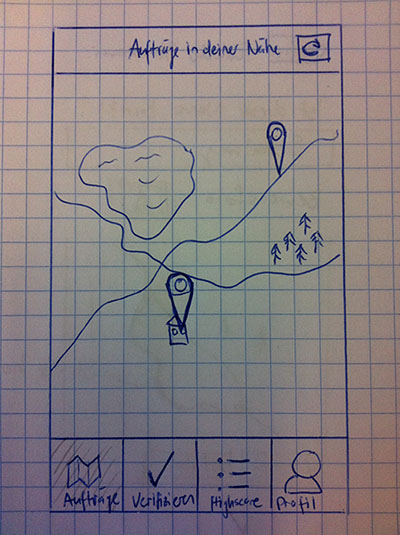
\includegraphics[width=0.43\textwidth]{images/paperprototype/kort-pp-bugs}}
\hfill
\subfigure[Aufträge - Detailansicht eines Fehlers]{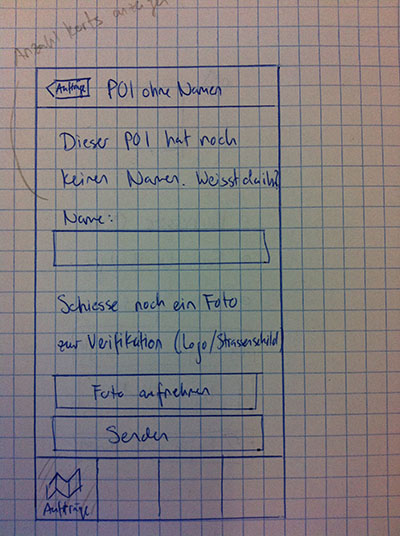
\includegraphics[width=0.43\textwidth]{images/paperprototype/kort-pp-fix}}
\end{figure}

\subsubsection{Maske: Verifizieren}
Auf der Verifikationsmaske werden die bereits gelösten Fehler in der Nähe angezeigt.
Sie sind gruppiert nach Anzahl nötigen Verifikationen, um sie zu OpenStreetMap zurückzusenden.

Per Klick auf einen Eintrag öffnet sich die Verifikationsmaske.
Darin wird der Fehlerlösungstext und das Beweis-Foto angezeigt.
Zusätzlich wird das betroffene OpenStreetMap-Objekt auf einer Karte angezeigt.
Man hat die Möglichkeit die Problemlösung als \emph{Korrekt} oder \emph{Falsch} zu werten.

\begin{figure}[H]
\subfigure[Verifizieren - Liste mit Fehlerlösungen]{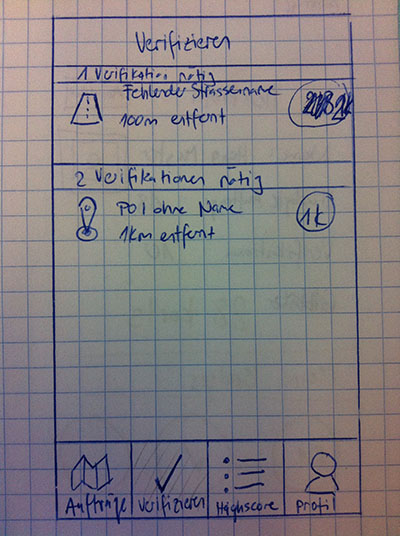
\includegraphics[width=0.43\textwidth]{images/paperprototype/kort-pp-verify}}
\hfill
\subfigure[Verifizieren - Detailansicht einer Fehlerlösung]{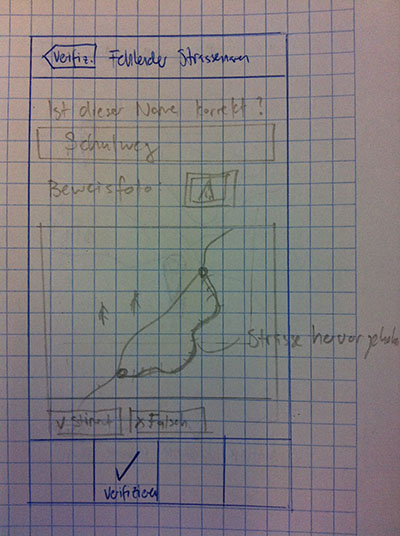
\includegraphics[width=0.43\textwidth]{images/paperprototype/kort-pp-verify_detail}}
\end{figure}

\subsubsection{Masken: Highscore / Profil}
In der Highscore-Maske hat man die Möglichkeit sich mit anderen Spielern vergleichen.
Man sieht seine eigene und die Platzierungen der anderen Spieler.
Es werden Highscores für verschiedene Kategorien (z.B. Regional, Weltweit) angezeigt.

Im Profil sieht man einen Steckbrief seines eigenen Benutzers.
Es wird angezeigt wieviele Aufträge man gelöst und wieviele Verifikationen man getätigt hat.
Zusätzlich werden die Gesamtanzahl der gesammelten Punkte und die gewonnenen Badges angezeigt.
Die Profil-Maske bietet zudem die Möglichkeit sich von der App abzumelden.

\begin{figure}[H]
\subfigure[Highscore]{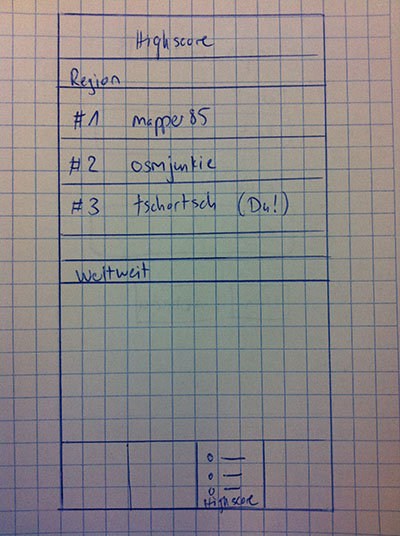
\includegraphics[width=0.43\textwidth]{images/paperprototype/kort-pp-highscore}}
\hfill
\subfigure[Profil]{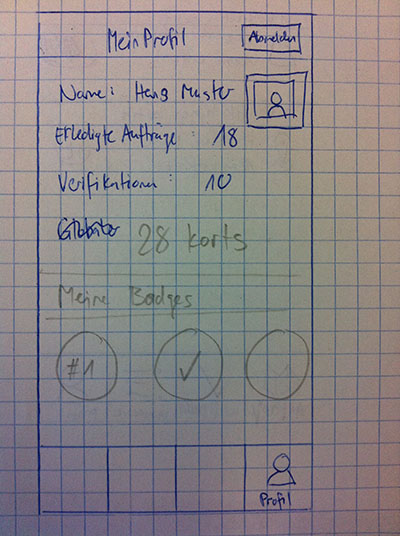
\includegraphics[width=0.43\textwidth]{images/paperprototype/kort-pp-profile}}
\end{figure}